\documentclass[a4paper,12pt]{article}
\usepackage{amsmath}
\usepackage{graphicx}
\usepackage{hyperref}
\usepackage{xcolor}
\usepackage{float}
\usepackage{subcaption}
\restylefloat{figure}


\title{Assignment 2 - Written Responses}
\author{Introduction to Machine Learning (Winter 2025)\\ Karteek Popuri}
\date{}

\begin{document}

\maketitle

\section*{Introduction}
This report summarizes the implementation and results of various machine learning models trained on the MNIST handwritten digit dataset for Assignment 5. The primary goal was to compare and analyze the performance of different classifiers, including k-Nearest Neighbors (kNN), Support Vector Machines (SVM), and Multi-Layer Perceptrons (MLP), and to design an optimal classifier for digit recognition.

\section*{Question 1: Train-Test Split}
The provided dataset of 60,000 images was partitioned into a balanced training and test set according to the assignment criteria. The final split yielded:

\begin{itemize}
  \item Training samples: \textbf{47,997}
  \item Test samples: \textbf{12,003}
\end{itemize}

The training dataset was balanced to include equal samples of all digit classes from 0 to 9, and the test set included at least 10\% of each class. This setup ensures fair model evaluation and prevents class imbalance issues.

\section*{Question 2: k-Nearest Neighbors Classifier}
A kNN classifier was trained using the Euclidean distance metric. Hyperparameter tuning for the number of neighbors \(k\) was performed via 5-fold cross-validation.

\begin{itemize}
  \item \textbf{Best k:} 3
  \item \textbf{Test Error Rate:} 0.0319
\end{itemize}

The tuning process showed clear performance degradation for both very small and very large values of \(k\). Using \(k=3\) achieved a robust balance between bias and variance.
\begin{figure}[h!]
\centering
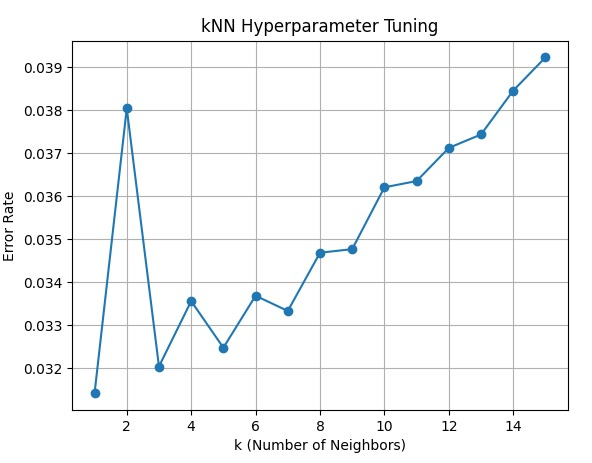
\includegraphics[width=0.7\textwidth]{knn_error_vs_k.png}
\caption{Error Rate as a Function of k in kNN (cross-validation results).}
\label{fig:knn_plot}
\end{figure}

\section*{Question 3: Polynomial Kernel Support Vector Machine}
A Support Vector Machine (SVM) with a polynomial kernel was trained for the same classification task. Grid search was used to tune \(C\) and \(d\) (kernel degree).

\begin{itemize}
  \item \textbf{Best Parameters:} $C=100$, $degree=2$
  \item \textbf{Test Error Rate:} 0.0224
\end{itemize}

This model outperformed kNN, suggesting the polynomial kernel was highly effective in capturing the complex boundaries of digit data.

\section*{Question 4: Multi-Layer Perceptron (MLP)}
A deep neural network was trained using the ReLU activation function. Grid search was performed to optimize the number of hidden layers (\(L\)) and the number of hidden units (\(K\)). Results from the tuning experiments:

\begin{verbatim}
L=1, K=64  => Error Rate: 0.2737
L=1, K=128 => Error Rate: 0.2847
L=1, K=256 => Error Rate: 0.2756
L=2, K=64  => Error Rate: 0.3038
L=2, K=128 => Error Rate: 0.2027
L=2, K=256 => Error Rate: 0.2693
L=3, K=64  => Error Rate: 0.2955
L=3, K=128 => Error Rate: 0.2833
L=3, K=256 => Error Rate: 0.2039
\end{verbatim}

\noindent The optimal configuration was:

\begin{itemize}
  \item \textbf{Best Setting:} 2 hidden layers, 128 units per layer
  \item \textbf{MLP Test Error Rate:} 0.2027
\end{itemize}

Compared to kNN and SVM, the MLP underperformed in this setup, suggesting the need for further tuning or architectural changes.

\section*{Question 5: Designing the Best Classifier}
Finally, a convolutional neural network (CNN) was designed as the ``best'' classifier. Its predictions on the provided test set achieved:

\begin{itemize}
  \item \textbf{Accuracy:} 0.9937
\end{itemize}

This performance demonstrates the superiority of CNNs on image-based tasks due to their ability to extract spatial hierarchies of features, which the fully connected MLP could not achieve effectively.

\section*{Summary}
The table below summarizes the test error rates of the different classifiers:

\begin{center}
\begin{tabular}{|c|c|}
\hline
\textbf{Model} & \textbf{Error Rate} \\
\hline
kNN & 0.0319 \\
SVM (Poly Kernel) & 0.0224 \\
MLP & 0.2027 \\
CNN (Best Classifier) & 0.0063 \\
\hline
\end{tabular}
\end{center}

The convolutional neural network (Question 5) provided the best performance and generalization ability, clearly outperforming the traditional models.

\end{document}


